\documentclass{beamer}

\usepackage[utf8]{inputenc}
\usepackage[T1]{fontenc}
\usepackage{textpos}
\usepackage{tikz}

\usetheme{Madrid}
\usecolortheme{beaver}

% Custom changes:
\setbeamertemplate{footline}[frame number]{}
\definecolor{university_tuebingen}{RGB}{165,30,55}
\setbeamercolor{frametitle}{fg=university_tuebingen, bg=white}
\setbeamercolor{title}{fg=university_tuebingen}

\addtobeamertemplate{frametitle}{}{
\begin{tikzpicture}[remember picture, overlay]
\node[anchor=north east,yshift=0cm] at (current page.north east)
{
\includegraphics[width=3cm]{../common/logo_uni_tuebingen2.png}};
\end{tikzpicture}}



\author{Prof. Dr. Christiane Zarfl, Dipl.-Inf. Willi Kappler}
%\date{\today}
\date{}
%\institute{Universität Tübingen}
\institute{}


\title{{
\beamertemplatenavigationsymbolsempty % suppress navigation on this (= first) slide
\begin{frame}[plain] % plain means: no header and footer on this (= first) slide
    \begin{textblock*}{0cm}(0.5cm, -0.7cm)
        
\includegraphics[width=11.0cm]{../common/logo_uni_tuebingen.png}
    \end{textblock*}
    \titlepage
    \begin{textblock*}{0cm}(0.1cm, -2.5cm)
        \textcolor{university_tuebingen}{\rule{11.8cm}{0.2cm}}
    \end{textblock*}
\end{frame}
}
\\{\scriptsize 1. Grundlagen}}

\begin{document}
    {
\beamertemplatenavigationsymbolsempty % suppress navigation on this (= first) slide
\begin{frame}[plain] % plain means: no header and footer on this (= first) slide
    \begin{textblock*}{0cm}(0.5cm, -0.7cm)
        
\includegraphics[width=11.0cm]{../common/logo_uni_tuebingen.png}
    \end{textblock*}
    \titlepage
    \begin{textblock*}{0cm}(0.1cm, -2.5cm)
        \textcolor{university_tuebingen}{\rule{11.8cm}{0.2cm}}
    \end{textblock*}
\end{frame}
}


    \section{Einleitung}
    \begin{frame}
      \frametitle{Inhaltsverzeichnis}
      \tableofcontents[currentsection]
    \end{frame}

    \subsection{Warum Matlab ?}
    \begin{frame}
      \frametitle{Matlab - Warum ?}
      \begin{textblock*}{0cm}(5.0cm, -1.0cm)
        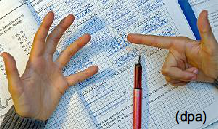
\includegraphics[width=3.0cm]{rechnen1.png}
      \end{textblock*}
      \begin{textblock*}{0cm}(9.0cm, 0.0cm)
        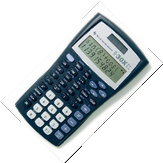
\includegraphics[width=2.0cm]{rechnen2.png}
      \end{textblock*}

      \begin{itemize}
        \itemsep0.4cm
        \item Einfache Rechnungen
        \item Datenaufbereitung \& -speicherung
        \item Visualisierung von Daten \& Simulationsergebnissen
        \item einfaches Lösen von (linearen) Gleichungssystemen, Differentialgleichungen (DGL), DGL-Systemen...
        \item Wiederverwendung von häufig gebrauchten Berechnungen (Programmierung)
        \item Datenanalyse (z.B. Regression) \& Statistik
        \item Komplexe Modellierung von Umweltsystemen
      \end{itemize}
    \end{frame}

    \subsection{Visualisierung}
    \begin{frame}
      \frametitle{Matlab - Warum ?}
      \vspace{-0.8cm}
      \begin{figure}
        Visualisierung von Daten \& Simulationsergebnissen \par \vspace{0.4cm}
        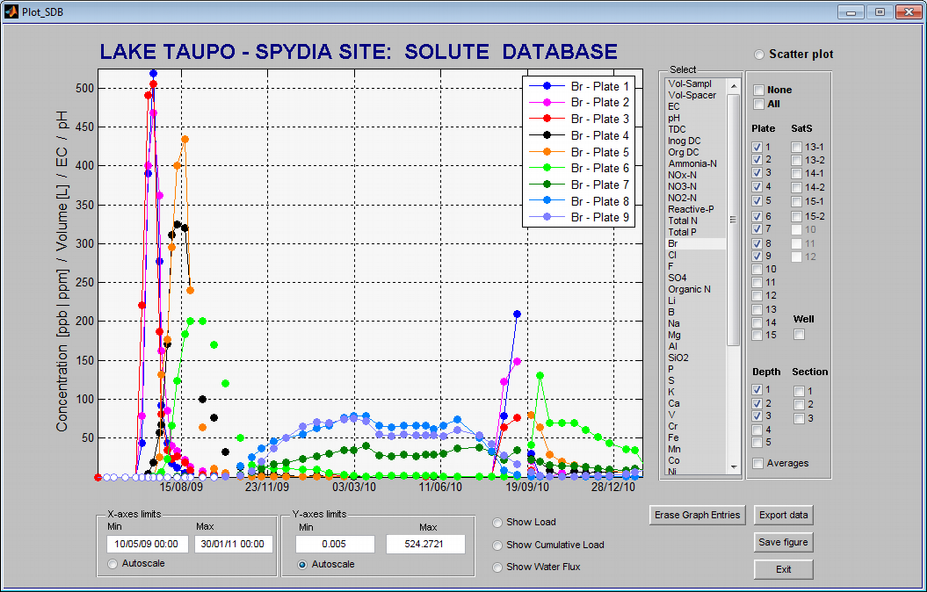
\includegraphics[width=10.0cm]{visualisierung1.png}
      \end{figure}
    \end{frame}

    \subsection{Datenalalyse}
    \begin{frame}
      \frametitle{Matlab - Warum ?}

      \vspace{-0.8cm}

      \begin{figure}
        Datenanalyse \& Statistik \par \vspace{0.4cm}
        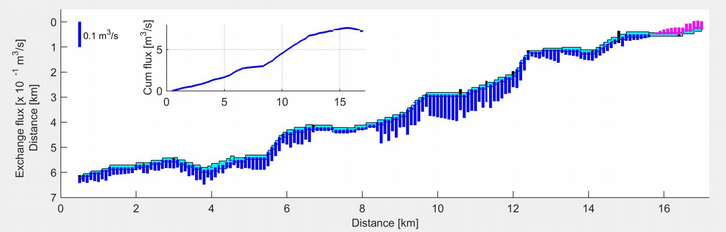
\includegraphics[width=10.0cm]{visualisierung2.png}
      \end{figure}

      \vspace{-0.5cm}

      \begin{figure}
        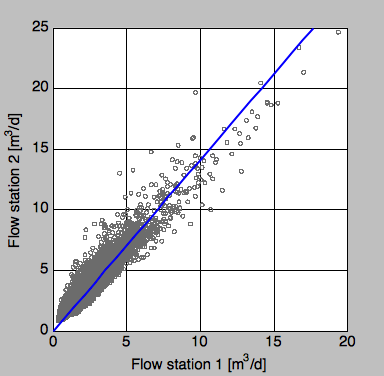
\includegraphics[width=3.0cm]{visualisierung3.png}
        \hspace{0.5cm}
        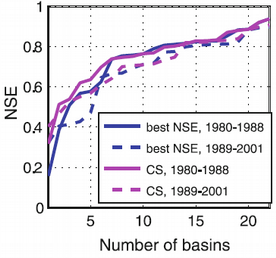
\includegraphics[width=3.0cm]{visualisierung5.png}
        \hspace{0.5cm}
        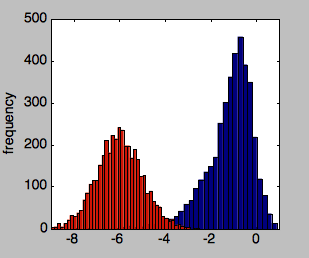
\includegraphics[width=3.0cm]{visualisierung4.png}
      \end{figure}
    \end{frame}

    \subsection{Modellierung}
    \begin{frame}
      \frametitle{Matlab - Warum ?}
      \vspace{-0.8cm}
      \begin{figure}
        Modellierung von Umwelstsystemen \par \vspace{0.4cm}
        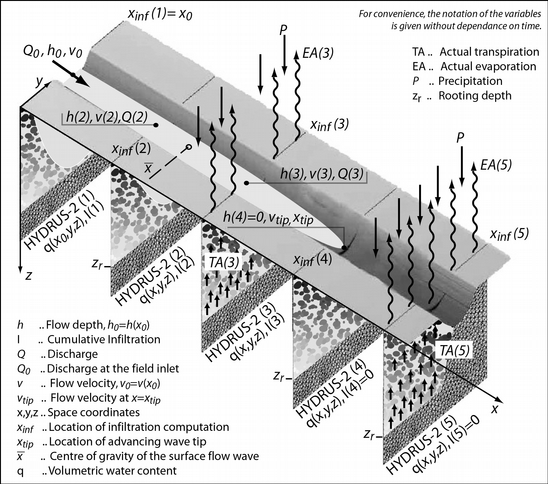
\includegraphics[width=7.5cm]{modellierung1.png}
      \end{figure}
    \end{frame}

    \subsection{Organisatorisches}
    \begin{frame}
        \frametitle{Organisatorisches}

        \vspace{-1.0cm}

        \begin{itemize}
          \item Hardware:

          \begin{itemize}
            \itemsep0.3cm
            \item BYOD (eigenes Gerät mitbringen)
            \item Geo-Notebooks (Raum S245)
            \item CIP Pool Rechner (Raum S310)
          \end{itemize}

          \item Software:

          \begin{itemize}
            \itemsep0.3cm
            \item Auf Institutshardware bereits vorinstalliert
            \item ZDV: Matlab herunterladen \href{https://services.zdv.uni-tuebingen.de/CampusSoftware/}{\beamergotobutton{Link}}
            \item GNU Octave \href{https://www.gnu.org/software/octave/}{\beamergotobutton{Link}} (Open Source, aber nicht 100\% compatibel)
          \end{itemize}

          \item \alert{Auf Institutshardware bitte zuerst ein eigenes Verzeichnis anlegen!}

        \end{itemize}
    \end{frame}

    \subsection{Was ist Matlab}
    \begin{frame}
        \frametitle{Was ist Matlab}

        \begin{itemize}
          \item "\emph{Matlab} ist eine kommerzielle Software des Unternehmens \emph{The MathWorks, Inc.} zur Lösung mathematischer Probleme
          und zur grafischen Darstellung der Ergebnisse." (Quelle: \href{https://de.wikipedia.org/wiki/Matlab}{\beamergotobutton{Wikipedia}}).
          \item Matlab leitet sich ab von \textbf{MAT}rix \textbf{LAB}oratory.
          \item Wir benutzen Matlab als (nummerische) Programmiersprache.
          \item Wie ein Taschenrechner oder Excel arbeitet Matlab nummerisch (mit Zahlenwerten, also nicht symbolisch wie
          ein \href{https://de.wikipedia.org/wiki/Computeralgebrasystem}{\beamergotobutton{CAS}}).
          \item Anders als bei einem Taschenrechner können Zahlenwerten Variablennamen zugewiesen werden.
          \item Im Programm werden die Variablennamen als Platzhalter für die Werte verwendet.
        \end{itemize}
    \end{frame}

    \subsection{Ausblick}
    \begin{frame}
        \frametitle{Nach diese ersten Kurseinheit...}

        \begin{itemize}
          \itemsep0.3cm
          \item kennen Sie den Aufbau der Oberfläche der Software Matlab.
          \item benutzen Sie die Matlab-Hilfe, um für Sie nützliche Funktionen und Informationen selbstständig zu finden.
          \item führen Sie einfache Rechnungen mit Matlab durch.
          \item können Sie Variablen in Matlab definieren und verwenden.
          \item kennen Sie die Vorteile der Verwendung von Vektoren und können diese in Matlab definieren und für Rechnungen verwenden.
        \end{itemize}
    \end{frame}

    \subsection{GUI}
    \begin{frame}
        \frametitle{Die Matlab GUI}
        \vspace{-0.8cm}
        \begin{figure}
          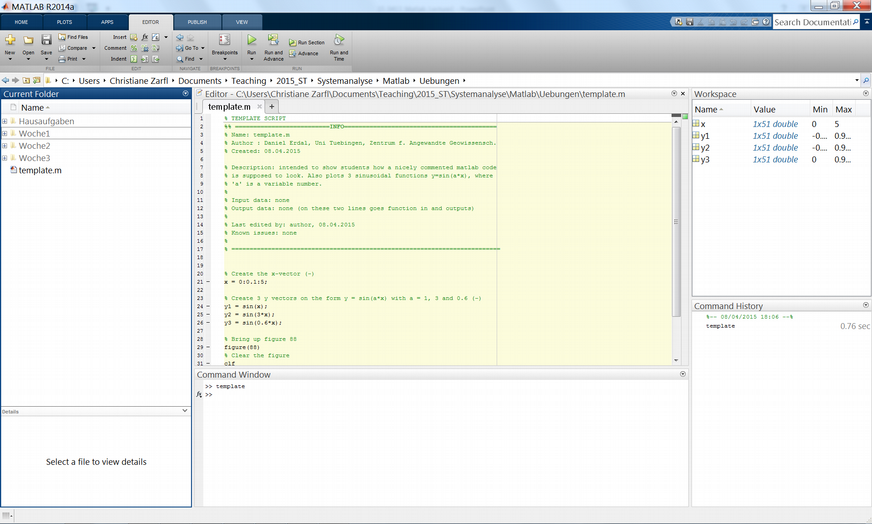
\includegraphics[width=10.0cm]{matlab_gui1.png}
        \end{figure}
    \end{frame}




    \section{Part 1}
    \begin{frame}
        \frametitle{This is the first slide}
        \begin{columns}[t]
          \begin{column}{5cm}
            \begin{exampleblock}{Matlab Code:}
              \lstinputlisting[language=Matlab]{example1.1.m}
            \end{exampleblock}
          \end{column}
          \begin{column}{5cm}
            \begin{block}{Ergebnis:}
              \lstinputlisting[language=Matlab]{example1.1.txt}
            \end{block}
          \end{column}
        \end{columns}

    \end{frame}

    \section{Part 2}
    \begin{frame}
        \frametitle{This is the second slide}
        \framesubtitle{A bit more information about this}
        Text
    \end{frame}
\end{document}
